%!TEX root = thesis.tex

\chapter{Conceptual Design of a TinyMLOps Ecosystem}
\label{chp:Framework}

Building upon the comprehensive analysis of the existing research landscape presented in Chapter~\ref{chp:Research_Results}, which highlighted notable gaps and identified pressing requirements, this chapter introduces the conceptual design of a novel, integrated ecosystem for autonomous \gls{tinymlops}. This ecosystem is composed of two primary, synergistic components: \gls{tinylcm}, an on-device framework engineered for autonomous machine learning lifecycle management on resource-constrained hardware, and TinySphere, an optional, yet deeply integrated, server-side platform designed to provide enhanced MLOps capabilities tailored to the specific needs of TinyML deployments. The subsequent sections will delineate the motivation and design rationale underpinning this ecosystem, articulate its core requirements and architectural vision, and provide a detailed exposition of both \gls{tinylcm} and TinySphere. This chapter directly addresses RQ3, which seeks to determine how a \gls{tinymlops} framework can be designed to enable effective on-device model lifecycle management in resource-constrained systems.

~\\
\vfill
\minitoc
\clearpage


\section{Motivation and Design Rationale}
\label{sec:framework_motivation_rationale}

The effective operationalization of \gls{ml} models on severely resource-constrained edge devices presents a distinct set of challenges that traditional \gls{mlops} paradigms, conceived for cloud-centric environments, do not adequately address. The systematic literature investigation in Chapter~\ref{chp:Research_Results} underscored several critical deficiencies in current TinyML practices and platforms. These identified limitations serve as the primary impetus for the development of the proposed TinyMLOps ecosystem, guiding its design rationale and architectural choices.

\subsection{Revisiting Research Gaps and Limitations}
\label{ssec:framework_revisiting_gaps}

The findings from Chapter~\ref{chp:Research_Results} (Sections~\ref{sec:RQ1_Results_SystemArchitecture} and \ref{sec:RQ2_Results_Frameworks}) revealed a fragmented landscape in TinyML operations. While individual solutions address specific aspects of the \gls{ml} lifecycle, a cohesive, end-to-end framework explicitly designed for \textit{autonomous} on-device lifecycle management remains largely elusive. Many contemporary approaches exhibit a significant reliance on cloud infrastructure for critical MLOps tasks such as model monitoring, retraining, and update deployment \cite{kreuzbergerMachineLearningOperations2023, antoniniTinyMLOpsFrameworkOrchestrating2022}. This dependency inherently limits the operational autonomy of edge devices, particularly in scenarios characterized by intermittent or non-existent connectivity—a common constraint in many real-world TinyML applications, exemplified by the Mars rover case study motivating this thesi

Furthermore, existing platforms, while powerful in their respective domains, often fall short of meeting the holistic requirements of managing adaptive, autonomous TinyML fleets. For instance, platforms like Edge Impulse excel in the initial development, optimization, and deployment phases of \gls{tinyml} models \cite{banburyEdgeImpulseMLOps2023}. However, their primary focus is less on the continuous, autonomous on-device adaptation and the operational management of numerous, independently evolving devices in the field. Similarly, generic \gls{mlops} tools such as MLflow, while offering robust capabilities for experiment tracking and model versioning in traditional settings, are not inherently designed for the nuances of TinyML, including extreme resource constraints, the need for on-device intelligence, or seamless interaction with device-specific lifecycle processes \cite{johnMLOpsFrameworkMaturity2021}. The literature also indicates a nascent stage in the integration of comprehensive device management capabilities within \gls{tinymlops} frameworks, a feature highlighted as beneficial in systems like SensiX++ \cite{minSensiXBringingMLOps2023}, yet not widely adopted. This points to a clear need for a server-side MLOps platform that is not merely an adaptation of cloud-centric tools but is purposefully architected to understand and augment autonomous on-device operations.

\subsection{Objectives and Core Tenets for the Proposed Ecosystem}
\label{ssec:framework_derived_objectives}

The identified research gaps and limitations directly inform the primary objectives and guiding principles for the proposed TinyMLOps ecosystem. The overarching goal is to empower resource-constrained edge devices with the capability for genuine operational autonomy throughout the \gls{ml} model lifecycle, while simultaneously providing an optional, yet synergistic, server-side infrastructure for enhanced management, validation, and oversight. This dual approach aims to strike a balance between on-device self-sufficiency and the benefits of centralized MLOps capabilities when connectivity and resources permit.

The design philosophy of the ecosystem is therefore "autonomy-first," where the on-device framework, \gls{tinylcm}, is engineered to perform all critical lifecycle functions independently. This includes continuous monitoring for concept drift without reliance on ground-truth labels, on-device model adaptation in response to detected changes, and robust state management. The server-side platform, TinySphere, is conceived as an optional, value-adding component that can ingest data and events from \gls{tinylcm} instances, offer advanced analytics, facilitate external validation of on-device adaptations, and provide fleet management functionalities.

In terms of architectural precedents identified in Chapter~\ref{chp:Research_Results} (Section~\ref{sec:RQ1_Results_SystemArchitecture}), the proposed ecosystem strategically combines proven patterns. For \gls{tinylcm}, a data-centric pipeline architecture is adopted, leveraging its prevalence and suitability for processing sequential data streams efficiently on edge devices. This choice facilitates modularity and a clear flow of operations from feature extraction to drift detection and adaptation. For the interaction between \gls{tinylcm} and TinySphere, a client-server model is employed. While seemingly contradictory to full autonomy, this pattern is implemented opportunistically, allowing \gls{tinylcm} to function independently and only engage with TinySphere when connectivity is available and beneficial. This server-side interaction is deemed crucial for realizing the full spectrum of MLOps capabilities, such as centralized logging, comparative performance analysis across a fleet, and human-in-the-loop validation, which are impractical or impossible for a single, isolated device to perform. The design of TinySphere itself specifically aims to address the identified lack of TinyML-centric MLOps platforms.


\section{System Requirements and High-Level Architectural Vision}
\label{sec:framework_requirements_vision}

To translate the derived objectives into a concrete design, a set of functional and non-functional requirements for the TinyMLOps ecosystem was established. These requirements are informed by the literature analysis, the overarching goal of enabling autonomous on-device \gls{ml} lifecycle management, and the specific challenges posed by the Mars rover case study. Following the articulation of these requirements, a high-level architectural vision for the complete ecosystem is presented.

\subsection{Functional and Non-Functional Requirements}
\label{ssec:framework_requirements}

The functional requirements (FR) define the core capabilities that the ecosystem must provide, while the non-functional requirements (NFR) specify the quality attributes essential for its effective operation in resource-constrained environments. These requirements are summarized in Table~\ref{tab:functional_requirements} and Table~\ref{tab:non_functional_requirements}.

\begin{table}[htbp]
    \caption[Functional Requirements for the TinyMLOps Ecosystem]{Functional Requirements for the TinyMLOps Ecosystem.}
    \label{tab:functional_requirements}
    \begin{tabularx}{\linewidth}{@{}lX@{}}
        \opentableheader
        \hl{ID} & \hl{Description} \\
        \closetableheader
        FR1 & \textbf{Autonomous On-Device Drift Detection:} The on-device component (\gls{tinylcm}) must be capable of continuously monitoring input data characteristics and/or model behavior to detect potential concept drift using proxy metrics, without requiring real-time ground truth labels. \\
        FR2 & \textbf{Informed On-Device Model Adaptation:} Upon detection of a potential drift, \gls{tinylcm} must provide mechanisms for immediate, yet cautious, on-device adaptation of the deployed \gls{ml} model, for instance, through heuristic-based pseudo-labeling or parameter adjustment. \\
        FR3 & \textbf{Robust On-Device State Management:} \gls{tinylcm} must implement robust state management, including versioning of models and relevant operational states, to enable rollbacks to previous stable states if an adaptation proves detrimental or an error occurs. \\
        FR4 & \textbf{Opportunistic Synchronization:} \gls{tinylcm} must support optional and opportunistic synchronization of its state, operational logs, detected drift events, and (pseudo-)labeled data with a designated server-side component (TinySphere). This synchronization must be resilient to intermittent connectivity. \\
        FR5 & \textbf{Server-Side Validation and Correction:} The server-side component (TinySphere) must be able to receive data from on-device instances and facilitate the (asynchronous) validation of on-device observations and heuristic adaptations, potentially providing corrected labels or model updates back to the device. \\
        FR6 & \textbf{Centralized Monitoring and Fleet Management:} TinySphere should provide capabilities for the centralized monitoring of a fleet of deployed devices, offering insights into their operational status, model performance, and encountered drift phenomena. \\
        FR7 & \textbf{Flexible Operational Modes:} The ecosystem must support distinct operational modes, ranging from purely autonomous on-device operation to fully server-assisted adaptive learning, configurable per device or application. \\
        \bottomrule
    \end{tabularx}
\end{table}

\begin{table}[htbp]
    \caption[Non-Functional Requirements for the TinyMLOps Ecosystem]{Non-Functional Requirements for the TinyMLOps Ecosystem.}
    \label{tab:non_functional_requirements}
    \begin{tabularx}{\linewidth}{@{}lX@{}}
        \opentableheader
        \hl{ID} & \hl{Description} \\
        \closetableheader
        NFR1 & \textbf{Resource Efficiency:} All on-device components (\gls{tinylcm}) must be optimized for minimal consumption of memory (RAM and flash), CPU cycles, and power, suitable for deployment on MCUs and low-power SBCs. \\
        NFR2 & \textbf{Modularity and Extensibility:} Both \gls{tinylcm} and TinySphere should be designed with a modular architecture, allowing for the easy extension or replacement of individual components (e.g., drift detection algorithms, classifiers, server-side analysis modules). \\
        NFR3 & \textbf{Scalability:} The server-side platform (TinySphere) must be designed to handle data and communication from a potentially large number of connected edge devices. \\
        NFR4 & \textbf{Reliability and Fault Tolerance:} The on-device framework must operate reliably under adverse conditions, and synchronization mechanisms must be fault-tolerant, capable of resuming after interruptions. \\
        NFR5 & \textbf{Configurability:} Key parameters of \gls{tinylcm}, such as drift detection sensitivity, adaptation strategies, and synchronization policies, must be configurable to suit diverse application needs and hardware capabilities. \\
        \bottomrule
    \end{tabularx}
\end{table}

\subsection{Overall Ecosystem Architecture}
\label{ssec:framework_overall_architecture}

The proposed TinyMLOps ecosystem is architecturally envisioned as a synergistic pairing of the on-device \gls{tinylcm} framework and the server-side TinySphere platform. \gls{tinylcm} acts as the intelligent agent on each edge device, endowed with the autonomy to manage the \gls{ml} model's lifecycle locally. TinySphere serves as an optional, centralized hub that enhances these on-device capabilities by providing robust backend support for MLOps processes that are impractical or inefficient to execute on individual constrained devices. This includes comprehensive data aggregation, advanced analytics, human-in-the-loop validation, and fleet-wide operational oversight.

Figure~\ref{fig:ecosystem_context_diagram} provides a high-level system context diagram illustrating the primary components and their interactions. \gls{tinylcm}, residing on the edge device, interfaces with local sensors and the deployed \gls{ml} model. It autonomously performs tasks such as feature processing, inference, drift detection, and model adaptation. Crucially, its `SyncClient` component manages opportunistic communication with the TinySphere API, transmitting packaged data (e.g., drift events, operational metrics, quarantined samples) and receiving feedback or updates. TinySphere, in turn, processes these incoming data packages, stores relevant information in its database (e.g., PostgreSQL) and object storage (e.g., MinIO), leverages external tools like MLflow for model registry and experiment tracking, and presents insights and management controls via a dashboard to ML engineers or data scientists.

\begin{figure}[htbp]
    \centering
    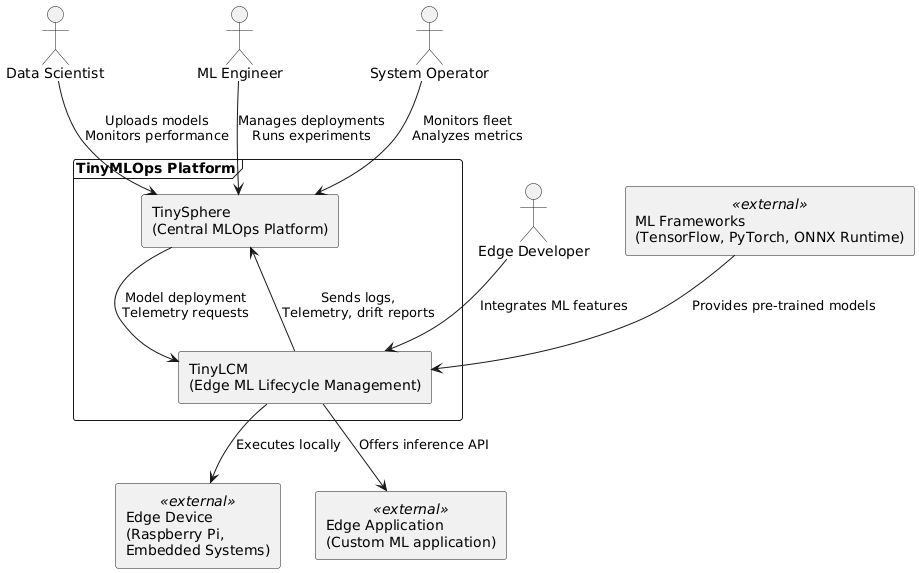
\includegraphics[width=0.975\textwidth]{figs/framework/system-context.png}
    \caption[High-Level System Context Diagram of the TinyMLOps Ecosystem]{High-Level System Context Diagram of the TinyMLOps Ecosystem, illustrating the interaction between Edge Devices (running \gls{tinylcm}) and the TinySphere Server.}
    \label{fig:ecosystem_context_diagram}
\end{figure}

The inherent design characteristic is that \gls{tinylcm} can fulfill its core mission of autonomous on-device lifecycle management even in the complete absence of TinySphere. However, the integration with TinySphere significantly augments its capabilities, transforming it from a standalone device solution into a component of a managed, adaptive, and evolving TinyML deployment. This architecture directly supports the required flexible operational modes (FR7), allowing a deployment to scale from fully disconnected autonomy to a comprehensively managed, server-assisted system.


\section{TinyLCM as On-Device Framework for Autonomous Lifecycle Management}
\label{sec:tinylcm_detailed_design}

At the heart of the proposed TinyMLOps ecosystem lies \gls{tinylcm}, a Python-based framework meticulously engineered to empower resource-constrained edge devices with autonomous \gls{ml} model lifecycle management capabilities. \gls{tinylcm} is designed to operate independently on devices such as Microcontroller Units (MCUs) and low-power Single-Board Computers (SBCs) like the Raspberry Pi Zero 2W. Its architecture and constituent components are optimized for resource efficiency, enabling on-device data processing, drift detection, model adaptation, and state management with minimal reliance on external infrastructure. This section provides a comprehensive exposition of \gls{tinylcm}'s architectural blueprint, its core on-device components, the mechanisms enabling autonomous operation, its resource-optimization strategies, and its interface for opportunistic communication.

\subsection{Architectural Blueprint and Core Components of TinyLCM}
\label{ssec:tinylcm_architecture_blueprint}

The architecture of \gls{tinylcm} is fundamentally data-centric and pipeline-oriented, facilitating a structured flow of data and control from input acquisition to decision-making and adaptation. It is composed of a core library (`/tinylcm`) containing the essential functionalities, and client tools (`/tinylcm/client`) for optional communication. Figure~\ref{fig:tinylcm_component_diagram} depicts the high-level component architecture of the \gls{tinylcm} core library.

\begin{figure}[htbp]
    \centering
    \includegraphics[width=0.975\textwidth]{figs/framework/tinylcm-component.png}
    \caption[Component Diagram of the TinyLCM Core Library]{Component Diagram of the \gls{tinylcm} Core Library, illustrating its main modules and their interdependencies.}
    \label{fig:tinylcm_component_diagram}
\end{figure}

The core library encompasses several key modules, detailed in Table~\ref{tab:tinylcm_core_modules}. These components are designed to be modular and configurable, often initialized based on JSON configuration files, allowing for flexibility in tailoring \gls{tinylcm} to specific applications and hardware.

\begin{itemize}
    \item \textit{Pipelines}: Orchestrate the overall workflow. The \texttt{InferencePipeline} manages basic inference and monitoring, while the \texttt{AdaptivePipeline} extends this with capabilities for on-device model adaptation, integrating components such as the \texttt{QuarantineBuffer} and \texttt{HeuristicAdapter}.
    \item \textit{Feature Extractors}: Responsible for deriving salient features from raw input data. A key implementation is the \texttt{TFLiteFeatureExtractor}, which leverages pre-trained TensorFlow Lite models (e.g., MobileNetV2) to extract high-dimensional feature vectors.
    \item \textit{Feature Transformers}: Process extracted features to optimize them for downstream tasks. The \texttt{StandardScalerPCATransformer} is a notable example, applying z-score standardization followed by Principal Component Analysis (PCA) for dimensionality reduction (1280D to 256D), which is crucial for efficient computation on constrained devices.
    \item \textit{Classifiers}: Perform the primary inference task. \gls{tinylcm} includes a \texttt{LightweightKNN} classifier, an optimized k-Nearest Neighbors implementation designed for low memory footprint and computational cost, capable of providing prediction confidence scores based on neighbor distances.
    \item \textit{Drift Detection Algorithms}: Implement various strategies for autonomous, on-device drift detection. Key detectors include \texttt{KNNDistanceMonitor}, \texttt{FeatureMonitor}, \texttt{PageHinkleyFeatureMonitor}, and \texttt{EWMAFeatureMonitor}, each targeting different statistical properties of the data or model behavior.
    \item \textit{State Management}: The \texttt{AdaptiveStateManager} is responsible for persisting and versioning the state of \gls{ml} models and other critical components. This enables robust operation and supports rollback capabilities.
    \item \textit{Data Logging and Adaptation Tracking}: These components facilitate the recording of operational data, inference results, detected drift events, and details of adaptation processes, which are vital for monitoring, debugging, and optional external validation.
    \item \textit{Operational Monitoring}: Tracks system-level metrics such as inference latency, CPU load, and memory usage, providing insights into the operational performance of the \gls{tinylcm} framework on the device.
    \item \textit{Heuristic Adaptation Components}: Part of the \texttt{AdaptivePipeline}, these manage samples flagged by drift detectors and implement heuristic-based pseudo-labeling for on-device model updates.
\end{itemize}.

\subsection{Lightwigth KNN Classifier}
\label{ssec:LightweightKNN}

Confidence Calculation for k-Nearest Neighbors:

\begin{lstlisting}[captionpos=b, language=Python, commentstyle=\color{blue}\itshape, caption=Distance-weighted confidence calculation for k-NN predictions,label=lst:confidenceCalc]
def calculate_confidence(neighbors):
    """Calculates class probabilities based on neighbor distances."""
    # Group neighbors by class and aggregate distances
    class_stats = {}
    for neighbor_idx, distance in neighbors:
        label = y_train[neighbor_idx]
        if label not in class_stats:
            class_stats[label] = {"count": 0, "total_distance": 0.0}
        class_stats[label]["count"] += 1
        class_stats[label]["total_distance"] += distance
    
    # Calculate adjusted probabilities
    adjusted_votes = {}
    total_adjusted_vote = 0.0
    
    for label, stats in class_stats.items():
        vote_prob = stats["count"] / k  # Base probability (vote fraction)
        avg_distance = stats["total_distance"] / stats["count"]
        distance_factor = 1.0 / (1.0 + scaling_factor * avg_distance)  # Penalize distance
        adjusted_vote = vote_prob * distance_factor  # Combined metric
        adjusted_votes[label] = adjusted_vote
        total_adjusted_vote += adjusted_vote
    
    # Normalize to probabilities
    probabilities = {
        label: vote / total_adjusted_vote 
        for label, vote in adjusted_votes.items()
    }
    return probabilities
\end{lstlisting}

\subsection{Autonomous Drift Detection and Adaptation Mechanisms}
\label{ssec:tinylcm_drift_adaptation}

A cornerstone of \gls{tinylcm}'s autonomy is its ability to detect and respond to concept drift without reliance on external ground truth labels. This is achieved through a sophisticated interplay of feature-space monitoring and heuristic-driven adaptation.

\subsubsection{Feature-Space Monitoring for Drift Detection}
\label{sssec:tinylcm_drift_theory}

Traditional drift detection methods often depend on the availability of true labels to monitor model performance, using ground truth verification \cite{disabatoTinyMachineLearning2024, pavanTyBoxAutomaticDesign2024}. However, in autonomous TinyML scenarios, such labels are not continuously available. To overcome this limitation, \gls{tinylcm} focuses on monitoring the statistical properties of the input data within a learned feature space. The underlying assumption is that concept drift often manifests as a change in the input data distribution $P(X)$ or the conditional probability $P(Y|X)$ \cite{gamaSurveyConceptDrift2014,disabatoTinyMachineLearning2024}. Changes in $P(X)$ can be detected by observing how new, incoming data points relate to a reference distribution of "normal" data established during a stable operational period.

The feature extraction process, typically employing a pre-trained deep neural network layer (e.g., from MobileNetV2), transforms raw input data into a high-dimensional feature space. Subsequent processing via standardization (using `StandardScaler` to achieve zero mean and unit variance) and PCA (Principal Component Analysis) serves multiple purposes: it normalizes feature scales, reduces dimensionality to mitigate the curse of dimensionality, retains the most variant (and often most informative) components, and can improve the robustness of distance-based metrics \cite{jolliffePrincipalComponentAnalysis2016,disabatoTinyMachineLearning2024}. Within this transformed, lower-dimensional feature space, the k-Nearest Neighbors (KNN) algorithm can be leveraged not only for classification but also as a tool for density estimation. The average distance to the k-nearest neighbors of a new data point can serve as a proxy for its conformity to the established data distribution; a significant increase in this average distance suggests that the new point is an outlier or originates from a drifted distribution \cite{chandolaAnomalyDetectionSurvey2009}. This unüberwacht approach is crucial for enabling autonomous drift detection on edge devices.

\subsubsection{KNN-Distance Monitoring with Page-Hinkley Test}
\label{sssec:tinylcm_knn_page_hinkley}

\gls{tinylcm}'s primary mechanism for autonomous drift detection in the \texttt{KNNDistanceMonitor} is based on continuously monitoring the average distance to the \(k\)-nearest neighbors in the PCA-transformed feature space.

Let \(\mathbf{f}_{\mathrm{raw}}\in\mathbb{R}^D\) denote the raw feature vector extracted from an input sample. This vector is first L\(^2\)-normalized to unit length in order to avoid biases due to differing magnitudes:
% Vorher: equation
\begin{flalign}
  && \mathbf{f}_{\mathrm{norm}}
  = \frac{\mathbf{f}_{\mathrm{raw}}}{\|\mathbf{f}_{\mathrm{raw}}\|_2},
  \qquad
  \|\mathbf{f}_{\mathrm{raw}}\|_2
  = \sqrt{\sum_{i=1}^D f_{\mathrm{raw},i}^2}. &&
  \label{eq:l2_norm}
\end{flalign}

Next, the normalized vector undergoes z-score standardization followed by a PCA transformation. From a historical reference dataset of normalized vectors \(X_{\mathrm{norm}}\in\mathbb{R}^{N\times D}\), a \texttt{StandardScaler} computes the per-feature means \(\boldsymbol{\mu}_{\mathrm{norm}}\) and standard deviations \(\boldsymbol{\sigma}_{\mathrm{norm}}\), and a \texttt{PCA} model determines the top \(K\) principal components collected in the projection matrix \(W\in\mathbb{R}^{D\times K}\). For a new normalized vector \(\mathbf{f}_{\mathrm{norm}}\), the transformations read
% Vorher: gather, jetzt flalign (jede Zeile bekommt eine Nummer)
\begin{flalign}
  && \mathbf{z}
  = \frac{\mathbf{f}_{\mathrm{norm}} - \boldsymbol{\mu}_{\mathrm{norm}}}
         {\boldsymbol{\sigma}_{\mathrm{norm}}}, &&
  \label{eq:z_score}\\
  && \mathbf{y}
  = \mathbf{z}\,W,
  \qquad
  \mathbf{y}\in\mathbb{R}^K. &&
  \label{eq:pca_transform}
\end{flalign}

The \texttt{LightweightKNN} component then identifies, for each new transformed point \(\mathbf{y}_t\in\mathbb{R}^K\), its \(k\)-nearest neighbors \(\{\mathbf{r}_1,\dots,\mathbf{r}_k\}\) from a reference set \(Y_{\mathrm{ref}} = \{\mathbf{y}_1^{\mathrm{ref}},\dots,\mathbf{y}_M^{\mathrm{ref}}\}\). The Euclidean distance to each neighbor is computed as
% Vorher: equation
\begin{flalign}
  && d(\mathbf{y}_t,\mathbf{r}_j)
  = \sqrt{\sum_{i=1}^K \bigl(y_{t,i} - r_{j,i}\bigr)^2}, &&
  \label{eq:euclidean_distance}
\end{flalign}
and the drift signal \(x_t\) is defined as the average of these distances:
% Vorher: equation
\begin{flalign}
  && x_t = \frac{1}{k}\sum_{j=1}^k d(\mathbf{y}_t,\mathbf{r}_j). &&
  \label{eq:drift_signal}
\end{flalign}

To detect a statistically significant and sustained increase in \(x_t\), the Page–Hinkley test is employed \cite{pageContinuousInspectionSchemes1954}. Given a reference mean distance \(\mu_0\) obtained during a warm-up phase and a small tolerance \(\delta>0\), the test statistics evolve as
% Vorher: gather, jetzt flalign (jede Zeile bekommt eine Nummer)
\begin{flalign}
  && m_t = m_{t-1} + \bigl(x_t - \mu_0 - \delta\bigr), \quad m_0 = 0, &&
  \label{eq:ph_mt}\\
  && M_t = \min\bigl(M_{t-1},\,m_t\bigr), \quad M_0 = 0, &&
  \label{eq:ph_Mt}\\
  && PH_t = m_t - M_t. &&
  \label{eq:ph_statistic}
\end{flalign}

A drift is declared when \(PH_t\) exceeds a predefined threshold \(\lambda\). To prevent rapid re-triggering, the \texttt{KNNDistanceMonitor} also uses an exit threshold \(\lambda_{\mathrm{exit}}\) and enforces a cooldown period.

\begin{figure}[htbp]
    \centering
    \includegraphics[width=0.65\textwidth]{figs/framework/knndistance-class.png}
    \caption[Class Diagramm KNNDistanceMonitor]{Class Diagram of the \texttt{KNNDistanceMonitor} component, illustrating its attributes and methods.}
    \label{fig:tinylcm-knndistance-class}
\end{figure}

\begin{algorithm}[htbp]
  \caption{Update procedure for the \texttt{KNNDistanceMonitor}}
  \label{alg:knn_distance_monitor_update}
  \begin{algorithmic}[1]
    \Require Current average KNN distance $x_t$; Reference mean $\mu_0$; Tolerance $\delta$; Detection threshold $\lambda$; Exit threshold $\lambda_{\mathrm{exit}}$; Current Page-Hinkley sums $m_{t-1}, M_{t-1}$; Warm-up data buffer $W$; Warm-up phase flag $is\_warmup$; Reference initialized flag $ref\_initialized$; In drift state flag $in\_drift\_state$.
    \If{$is\_warmup$}
      \State Add $x_t$ to $W$.
      \State \Return \textbf{no drift}
    \ElsIf{not $ref\_initialized$}
      \State $\mu_0 \gets \mathrm{mean}(W)$; $\sigma_0 \gets \mathrm{std}(W)$ \Comment{Initialize reference from warm-up data}
      \State $m_t \gets 0$; $M_t \gets 0$ \Comment{Initialize Page-Hinkley statistics}
      \State $ref\_initialized \gets \textbf{true}$
      \State \Return \textbf{no drift}
    \Else
      \State $m_t \gets m_{t-1} + (x_t - \mu_0 - \delta)$
      \State $M_t \gets \min(M_{t-1}, m_t)$
      \State $PH_t \gets m_t - M_t$
      \If{not $in\_drift\_state$ and $PH_t > \lambda$}
        \State $in\_drift\_state \gets \textbf{true}$
        \State \Return \textbf{drift detected}
      \ElsIf{$in\_drift\_state$ and $PH_t \le \lambda_{\mathrm{exit}}$}
        \State $in\_drift\_state \gets \textbf{false}$
        \State $m_t \gets 0$; $M_t \gets 0$ \Comment{Reset Page-Hinkley statistics}
        \State \Return \textbf{drift ended}
      \Else
        \State \Return \textbf{no drift (or still in drift)}
      \EndIf
    \EndIf
  \end{algorithmic}
\end{algorithm}

\subsubsection{Heuristic Pseudo-Labeling and Quarantine}
\label{sssec:tinylcm_heuristic_adaptation}

Upon the detection of a significant drift by components like the `KNNDistanceMonitor`, \gls{tinylcm}'s `AdaptivePipeline` initiates an on-device adaptation process. This process is designed to be immediate yet cautious, leveraging a heuristic-based pseudo-labeling strategy.

The first step in this process is the use of a \textit{Quarantine Buffer}. Samples that trigger a drift alert, or those immediately following it and exhibiting similar anomalous characteristics (e.g., high KNN distance), are temporarily moved to a \texttt{QuarantineBuffer}. This buffer serves to collect a small, manageable set of these "unusual" samples for further analysis.

Subsequently, \textit{Heuristic Pseudo-Labeling} is performed. The \texttt{HeuristicAdapter} component analyzes the feature vectors of samples within the \texttt{QuarantineBuffer}. A common heuristic employed involves clustering these quarantined samples in their PCA-transformed feature space. If a sufficiently distinct and cohesive cluster forms from these new, anomalous samples, it might be inferred that these samples represent a new, coherent concept. A pseudo-label can then be assigned to this cluster. For example, if the original model was trained to classify objects A and B, and a new cluster of quarantined samples emerges that is significantly distant from the known clusters for A and B, these samples could be heuristically pseudo-labeled as representing a "Concept C". The confidence associated with such a pseudo-label might be determined by factors such as the intra-cluster cohesion, the degree of separation from existing known classes, and the number of samples forming the new cluster. % TODO: Consider adding a simplified formula for a clustering heuristic or confidence score for pseudo-labels.

Following the generation of pseudo-labels, a \textit{Cautious Model Update} is executed. The \texttt{LightweightKNN} classifier is then incrementally updated by adding these pseudo-labeled samples to its reference set $Y_{\mathrm{ref}}$. The "cautious" nature of this adaptation is ensured by several factors: typically, only a small number of pseudo-labeled samples are added to the model at any one time; the adaptation is often localized to the KNN model, leaving the more computationally expensive feature extractor unchanged; and, critically, the system maintains a state snapshot prior to the update, enabling a potential rollback if the adaptation proves detrimental.

Finally, the process incorporates \textit{Opportunistic External Validation}. As will be detailed in the context of the \texttt{SyncClient}, these pseudo-labeled samples and the contextual information surrounding their generation are packaged for optional, asynchronous transmission to the TinySphere server platform. TinySphere can then employ more sophisticated validation methods, potentially involving human-in-the-loop analysis, to confirm or refute the heuristically assigned pseudo-labels. This externally validated feedback can subsequently be used to refine the on-device model more robustly, leading to more accurate and reliable long-term adaptation.


Figure~\ref{fig:adaptation_sequence_diagram} illustrates the sequence of operations during an autonomous on-device adaptation cycle.

\begin{figure}[htbp]
    \centering
    \includegraphics[width=0.75\textwidth]{figs/framework/sequenz-simplified.png}
    \caption[Sequence Diagram of On-Device Adaptation]{Sequence Diagram illustrating the on-device adaptation process in \gls{tinylcm} following a drift detection.}
    \label{fig:adaptation_sequence_diagram}
\end{figure}

\subsubsection{State Management for Resilience}
\label{sssec:tinylcm_state_management}

To ensure operational resilience, particularly in the context of autonomous adaptations that might not always be beneficial, \gls{tinylcm} incorporates a robust `AdaptiveStateManager`. This component is responsible for versioning the state of critical elements, most notably the `LightweightKNN` classifier's reference set ($Y_{ref}$ and associated labels/timestamps).

Before an on-device adaptation (i.e., adding pseudo-labeled samples to the KNN), the `AdaptiveStateManager` saves the current state of the classifier. This typically involves serializing the feature vectors and labels of the KNN's reference samples, along with a version identifier and timestamp, to a non-volatile storage area on the device (e.g., a designated partition in flash memory, managed to minimize write amplification). If a subsequent evaluation (either through on-device monitoring of proxy metrics or via feedback from TinySphere) indicates that an adaptation has degraded performance, \gls{tinylcm} can trigger a rollback. This involves the `AdaptiveStateManager` restoring the classifier to its previously saved, known-good state. The state manager also handles pruning old versions to manage limited storage space. This mechanism (FR3) is crucial for maintaining system reliability when operating autonomously with heuristic-based learning.

\section{TinySphere: A TinyML-Centric Server Platform for Enhanced MLOps}
\label{sec:tinysphere_detailed_design}

While \gls{tinylcm} provides the foundation for on-device autonomy, the TinySphere platform serves as its optional, server-side counterpart, designed to offer enhanced MLOps capabilities specifically tailored to the nuances of managing fleets of adaptive TinyML devices. TinySphere is not merely a generic MLOps backend; it is architected to seamlessly integrate with \gls{tinylcm}, understand its operational data, and provide functionalities that augment on-device intelligence. This section outlines the rationale for TinySphere, its architectural design, and its key contributions to the overall TinyMLOps ecosystem.

\subsection{Rationale and Objectives for a TinyML-Centric MLOps Platform}
\label{ssec:tinysphere_rationale}

The development of TinySphere is motivated by the observation (Section~\ref{ssec:framework_revisiting_gaps}) that existing MLOps platforms, including powerful tools like Edge Impulse for model creation or MLflow for generic experiment tracking, do not fully cater to the operational lifecycle management of *autonomous, adaptive fleets of TinyML devices*. While Edge Impulse excels at the initial design and deployment stages, and MLflow offers robust components for traditional MLOps, a dedicated platform is needed to:

\begin{itemize}
    \item Process and interpret the unique data streams originating from \gls{tinylcm}-enabled devices (e.g., drift events, pseudo-labeled samples, on-device adaptation logs).
    \item Facilitate the external validation of on-device heuristic adaptations, a crucial step for ensuring the long-term reliability of autonomous learning.
    \item Provide centralized monitoring and comparative analytics across a distributed fleet of resource-constrained devices.
    \item Offer tailored model management and deployment strategies that account for the specific constraints and capabilities of TinyML targets.
\end{itemize}

TinySphere aims to fill this gap by providing a cohesive server environment that complements \gls{tinylcm}'s on-device autonomy with centralized oversight, validation, and advanced MLOps functionalities.

\subsection{Architectural Design of TinySphere}
\label{ssec:tinysphere_architecture}

TinySphere is implemented as a modern web application with a backend built using FastAPI, providing a robust and scalable RESTful API for communication with \gls{tinylcm} clients. For data persistence, it utilizes a PostgreSQL database for structured metadata (e.g., device information, drift event details, processed metrics) and MinIO (an S3-compatible object storage solution) for storing larger artifacts such as images associated with drift events, prediction snapshots, and extensive operational logs. Figure~\ref{fig:tinysphere_technical_diagram} presents a simplified technical context diagram of TinySphere's architecture.

\begin{figure}[htbp]
    \centering
    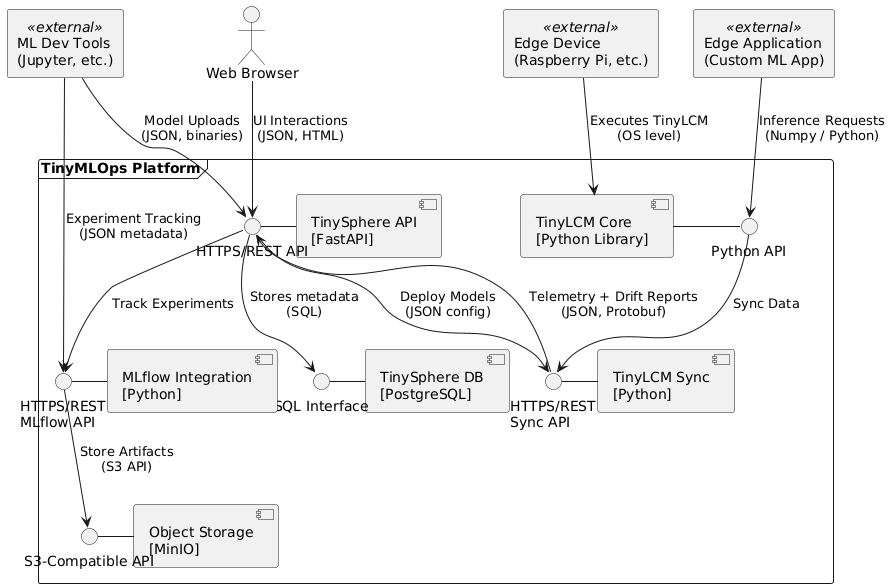
\includegraphics[width=0.975\textwidth]{figs/framework/technical-context.png}
    \caption[Technical Architecture of the TinySphere Server Platform]{Technical Architecture of the TinySphere Server Platform.}
    \label{fig:tinysphere_technical_diagram}
\end{figure}

\subsection{Key MLOps Capabilities Provided by TinySphere}
\label{ssec:tinysphere_capabilities}

TinySphere extends the on-device capabilities of \gls{tinylcm} by providing the following server-side MLOps functionalities:

\begin{itemize}
    \item \textit{External Validation of On-Device Adaptations:} TinySphere receives data on drift events and heuristic pseudo-labels generated by \gls{tinylcm}. This allows human experts or more powerful server-side models to validate these on-device decisions. Confirmed labels or corrections can then be communicated back to the device, enabling more robust and accurate long-term adaptation.
    \item \textit{Centralized Monitoring and Fleet Overview:} The platform aggregates operational metrics, drift alerts, and model performance indicators from all connected devices, providing a centralized dashboard for monitoring the health and behavior of the entire TinyML fleet. This facilitates the identification of systemic issues or widespread drift patterns.
    \item \textit{Enhanced Data Logging and Analytics:} TinySphere provides persistent storage for extensive operational logs and rich contextual data (e.g., images associated with drift) that would be impractical to store long-term on resource-constrained devices. This historical data enables more profound offline analysis and debugging.
    \item \textit{Model Management and Deployment Support (via MLflow Integration):} While \gls{tinylcm} handles on-device state, TinySphere can integrate with tools like MLflow for a centralized model registry. This allows ML engineers to manage different versions of base models, track server-side retraining experiments initiated based on field data, and potentially orchestrate the deployment of new base models or configurations to devices through \gls{tinylcm}'s model pull mechanism. TinySphere acts as the TinyML-aware orchestrator around MLflow's generic capabilities.
    \item \textit{Geolocation-based Insights:} If devices report their location, TinySphere can correlate model performance and drift occurrences with geographical areas, providing spatial context to operational data.
\end{itemize}

\begin{figure}[htbp]
    \centering
    \includegraphics[width=0.975\textwidth]{figs/framework/ui-tinyssphere.png}
    \caption[User Interface of TinySphere]{User Interface of TinySphere, illustrating the dashboard for monitoring device status and drift events.}
    \label{fig:uitinysphere}
\end{figure}

\section{The TinyMLOps Ecosystem: Synergies and Operational Modes}
\label{sec:ecosystem_synergies_modes}

The efficacy of the proposed TinyMLOps solution stems from the synergistic interplay between the on-device intelligence of \gls{tinylcm} and the optional, enhancing capabilities of the TinySphere server platform. This architecture facilitates a spectrum of operational modes, catering to diverse application requirements regarding autonomy, connectivity, and management overhead. This section details this synergy, outlines a typical operational workflow, and discusses the supported operational modes.


\subsection{Synergistic Integration of TinyLCM and TinySphere}
\label{ssec:ecosystem_integration_philosophy}


The core design philosophy is "autonomy-first, enhanced optionally." \gls{tinylcm} is engineered to function as a completely autonomous edge ML system, capable of performing its entire lifecycle management locally without any dependency on server connectivity. TinySphere acts as an optional enhancement layer, providing enterprise-grade MLOps capabilities that augment, but do not compromise, this edge autonomy.

This design ensures:
\begin{itemize}[noitemsep, topsep=0pt]
    \item \textit{Independent Edge Operation:} \gls{tinylcm}-equipped devices perform inference, drift detection, heuristic adaptation, and local state management (including versioning and rollbacks) entirely on their own.
    \item \textit{Optional Cloud Enhancement:} When connectivity is available, \gls{tinylcm}'s \texttt{SyncClient} component can opportunistically transmit packaged data (logs, metrics, drift event details, quarantined samples with pseudo-labels) to TinySphere.
    \item \textit{Graceful Degradation:} If network connectivity is lost or TinySphere is unavailable, \gls{tinylcm} continues its autonomous operation seamlessly. The \texttt{SyncClient} queues data locally for later transmission when connectivity is restored.
    \item \textit{Scalable Deployment:} The ecosystem supports deployments ranging from single, fully offline devices to large, managed fleets interacting with TinySphere.
\end{itemize}

TinySphere complements \gls{tinylcm} by providing:
\begin{itemize}[noitemsep, topsep=0pt]
    \item \textit{Centralized Data Hub and Analytics:} Aggregation and analysis of data from multiple devices.
    \item \textit{MLflow Integration:} For experiment tracking and versioning of models that might be (re)trained or fine-tuned based on fleet-wide data.
    \item \textit{Drift Hub for Validation:} A crucial component where human operators or more sophisticated server-side models can validate drift events and pseudo-labels generated by \gls{tinylcm}, providing a feedback loop for improving on-device models (FR5).
    \item \textit{Device Fleet Management:} Monitoring the status, health, and software versions of deployed devices.
\end{itemize}

The \texttt{SyncClient} in \gls{tinylcm} is key to this resilient integration. It handles data packaging (e.g., into compressed TAR archives with metadata), manages an upload queue for offline resilience, and implements retry logic for transmissions. It can also perform initial device registration with TinySphere, providing platform details and potentially geolocation data if available and permitted.

\subsection{Exemplary Operational Workflow}
\label{ssec:ecosystem_workflow}

To illustrate the practical application of the ecosystem, an exemplary end-to-end workflow, particularly relevant for the Proof-of-Concept (POC) development and deployment, is outlined below. This workflow spans from local model development to production operation with MLOps integration. A detailed sequence diagram of the interactions is provided in Appendix~\ref{app:integration_sequence_diagram}.


\textbf{Phase 1: Local Development and Training}
\begin{enumerate}[noitemsep, topsep=0pt]
    \item \textit{Model Prototyping and Training:} On a local development machine, an ML engineer uses scripts to perform transfer learning (e.g., with MobileNetV2) on a custom dataset. This process generates a quantized \gls{tflm} model, associated labels, and a feature processing pipeline including StandardScaler and PCA components.
    \item \textit{Initial State Generation:} Scripts are used to create the initial \gls{knn} state and reference statistics required by \gls{tinylcm}'s drift detectors, using the trained model and feature processor.
    \item \textit{Configuration Preparation:} A scenario-specific JSON configuration file is prepared, defining the paths to these artifacts and parameters for \gls{tinylcm}'s components.
    \item \textit{Version Control:} All generated artifacts, configurations, and source code are committed to a Git repository.
\end{enumerate}

\textbf{Phase 2: Device Deployment and Autonomous Operation}
\begin{enumerate}[noitemsep, topsep=0pt]
    \item \textit{Edge Device Setup:} A Raspberry Pi Zero 2W (e.g., on the Mars rover prototype) is prepared with a base OS (e.g., Raspberry Pi OS Lite).
    \item \textit{One-Line Installation:} The device executes an installation script (fetched from the GitHub repository via `curl`). This script clones the repository, installs necessary dependencies, copies the \gls{tinylcm} library and the specific scenario files (including models and configurations) to the device, and sets up the required directory structure.
    \item \textit{Autonomous Execution:} The main application script is started on the device. \gls{tinylcm} begins its autonomous operation: performing inference, continuously monitoring for drift, managing its local state, and potentially performing heuristic adaptations if drifts are detected. All significant events are logged locally.
\end{enumerate}

\textbf{Phase 3: Optional TinySphere Integration and MLOps}
\begin{enumerate}[noitemsep, topsep=0pt]
    \item \textit{Opportunistic Synchronization:} If configured and network connectivity is available, \gls{tinylcm}'s \texttt{SyncClient} periodically packages local logs, operational metrics, drift event data (including associated images or features), and pseudo-labeled samples. These packages are transmitted to the TinySphere API.
    \item \textit{Data Ingestion and Processing (TinySphere):} TinySphere's backend receives these packages. Its `PackageImporter` component extracts the data and routes it to appropriate services:
        \begin{itemize}[noitemsep, topsep=0pt, leftmargin=1em]
            \item Operational logs and metrics are stored in PostgreSQL and MinIO.
            \item Drift event details, including quarantined samples and features, are processed by the `DriftTransformer` and stored, making them available in the Drift Hub (Figure~\ref{fig:uitinysphere_drifthub_example}a).
            \item Prediction images or features might be stored by a `PredictionImagesTransformer`.
        \end{itemize}
    \item \textit{MLflow Integration (TinySphere):} An `MLflowService` can process model-related information from the device packages or from server-side (re)training activities, logging experiments, parameters, metrics, and registering model versions in an MLflow tracking server, with artifacts stored in MinIO.
    \item \textit{Fleet Management and Monitoring (TinySphere):} ML engineers can use the TinySphere web interface (Figure~\ref{fig:uitinysphere_drifthub_example}b) to monitor the status of registered devices, view aggregated performance analytics, and examine drift events across the fleet.
    \item \textit{Ground Truth Validation (TinySphere Drift Hub):} Through the Drift Hub UI, human operators can review drift events, examine associated data (e.g., images of unknown objects), and provide ground truth labels. This validated information is stored and can create a feedback package for the originating device.
    \item \textit{Feedback Loop and Model Improvement:} When \gls{tinylcm} next syncs with TinySphere, it can retrieve this validated feedback. This feedback can be used to correct or confirm on-device pseudo-labels, refine the \gls{knn} model more accurately, or inform a central retraining cycle for the base feature extractor model if systemic drift is observed across multiple devices.
\end{enumerate}
This workflow enables a continuous cycle of deployment, autonomous operation, monitoring, validation, and improvement, embodying the core principles of MLOps adapted for the TinyML domain. Figure~\ref{fig:uitinysphere_drifthub_example} shows example mockups of how TinySphere's UI might support parts of this workflow. 


\begin{figure}[htbp]
    \centering % Zentriert die gesamte Figure-Umgebung

    % Erste Zeile mit zwei Subfigures
    \begin{subfigure}[b]{0.48\textwidth} % [b] für bottom alignment
        \centering
        \includegraphics[width=\textwidth]{figs/framework/device-page.png} % Dein Bild für Device Page
        \caption{TinySphere device page providing an overview of the device fleet, including status, key statistics, and location data for individual devices.}
        \label{fig:ui_device_page} % Eindeutiges Label
    \end{subfigure}
    \hfill % Flexibler horizontaler Abstand
    \begin{subfigure}[b]{0.48\textwidth}
        \centering
        \includegraphics[width=\textwidth]{figs/framework/model-page.png} % Dein Bild für Model Registry
        \caption{Model registry interface in TinySphere, listing available \gls{ml} models, their versions, and associated metadata for management.}
        \label{fig:ui_model_registry} % Eindeutiges Label
    \end{subfigure}

    \vspace{1em} % Vertikaler Abstand zwischen den Zeilen

    % Zweite Zeile mit zwei Subfigures
    \begin{subfigure}[b]{0.48\textwidth}
        \centering
        \includegraphics[width=\textwidth]{figs/framework/data-hub-page.png} % Dein Bild für Data Hub
        \caption{Data Hub view in TinySphere, illustrating the aggregation and accessibility of data collected from deployed \gls{tinylcm} devices.}
        \label{fig:ui_data_hub} % Eindeutiges Label
    \end{subfigure}
    \hfill
    \begin{subfigure}[b]{0.48\textwidth}
        \centering
        \includegraphics[width=\textwidth]{figs/framework/mlflow-page.png} % Dein Bild für MLflow Integration
        \caption{Integration with MLflow, showcasing tracked experiments and runs, including logged parameters, metrics, and artifacts.}
        \label{fig:ui_mlflow_integration} % Eindeutiges Label
    \end{subfigure}

    \vspace{1em} % Vertikaler Abstand zwischen den Zeilen

    % Dritte Zeile mit zwei Subfigures
    \begin{subfigure}[b]{0.48\textwidth}
        \centering
        \includegraphics[width=\textwidth]{figs/framework/minio-page.png} % Dein Bild für MinIO Integration
        \caption{MinIO object storage integration, displaying the bucket structure used for storing artifacts such as models, datasets, and logs.}
        \label{fig:ui_minio_integration} % Eindeutiges Label
    \end{subfigure}
    \hfill
    \begin{subfigure}[b]{0.48\textwidth}
        \centering
        \includegraphics[width=\textwidth]{figs/framework/api-page.png} % Dein Bild für OpenAPI Docs
        \caption{Integrated OpenAPI (Swagger) documentation for the TinySphere API, providing an interactive reference for developers.}
        \label{fig:ui_openapi_docs} % Eindeutiges Label
    \end{subfigure}

    \caption{Illustrative mockups of TinySphere User Interface components and integrations supporting the MLOps workflow: (a) Device fleet management page, (b) Model registry, (c) Data Hub, (d) MLflow experiment tracking, (e) MinIO bucket structure, and (f) OpenAPI documentation.}
    \label{fig:tinysphere_ui_examples_3x2} % Neues, eindeutiges Label für die gesamte Figure
\end{figure}

\subsection{Supported Operational Modes}
\label{ssec:ecosystem_operational_modes}

The dual architecture of \gls{tinylcm} and TinySphere inherently supports a range of operational modes (FR7), allowing deployments to be tailored to specific needs:

\begin{enumerate}[noitemsep, topsep=0pt]
    \item \textit{Fully Autonomous (Disconnected) Mode:} \gls{tinylcm} operates entirely on the edge device without any communication with TinySphere. All drift detection, adaptation, and state management are local. This mode is suitable for devices in permanently disconnected environments or where data exfiltration is prohibited.
    \item \textit{Autonomous with Opportunistic Synchronization Mode:} \gls{tinylcm} operates autonomously but periodically attempts to synchronize data with TinySphere when connectivity is available. This allows for offline data analysis, remote monitoring, and potential reception of validated feedback without compromising core on-device autonomy during periods of disconnection. This is the primary mode envisioned for the Mars rover scenario.
    \item \textit{Server-Assisted Adaptive Learning Mode:} In scenarios with more reliable connectivity, TinySphere can play a more active role. While \gls{tinylcm} still performs initial drift detection and heuristic adaptation, the validation of these adaptations and the triggering of more significant model updates (e.g., retraining or fine-tuning of the feature extractor) can be orchestrated or heavily guided by TinySphere based on aggregated fleet data and human expertise.
    \item \textit{Centralized Monitoring and Inference-Only Mode:} For less critical applications or where on-device adaptation is not desired, \gls{tinylcm} can be configured to perform only inference and drift monitoring, reporting all data to TinySphere, which then handles all analysis and decisions regarding model updates (which might be manually deployed or pushed).
\end{enumerate}
This flexibility allows the ecosystem to be applied to a wide spectrum of TinyML use cases, from highly autonomous systems to centrally managed fleets.
